\section{Evidence Accumulation Clustering}

\begin{frame}
\frametitle{Evidence Accumulation Clustering}

\begin{center}
    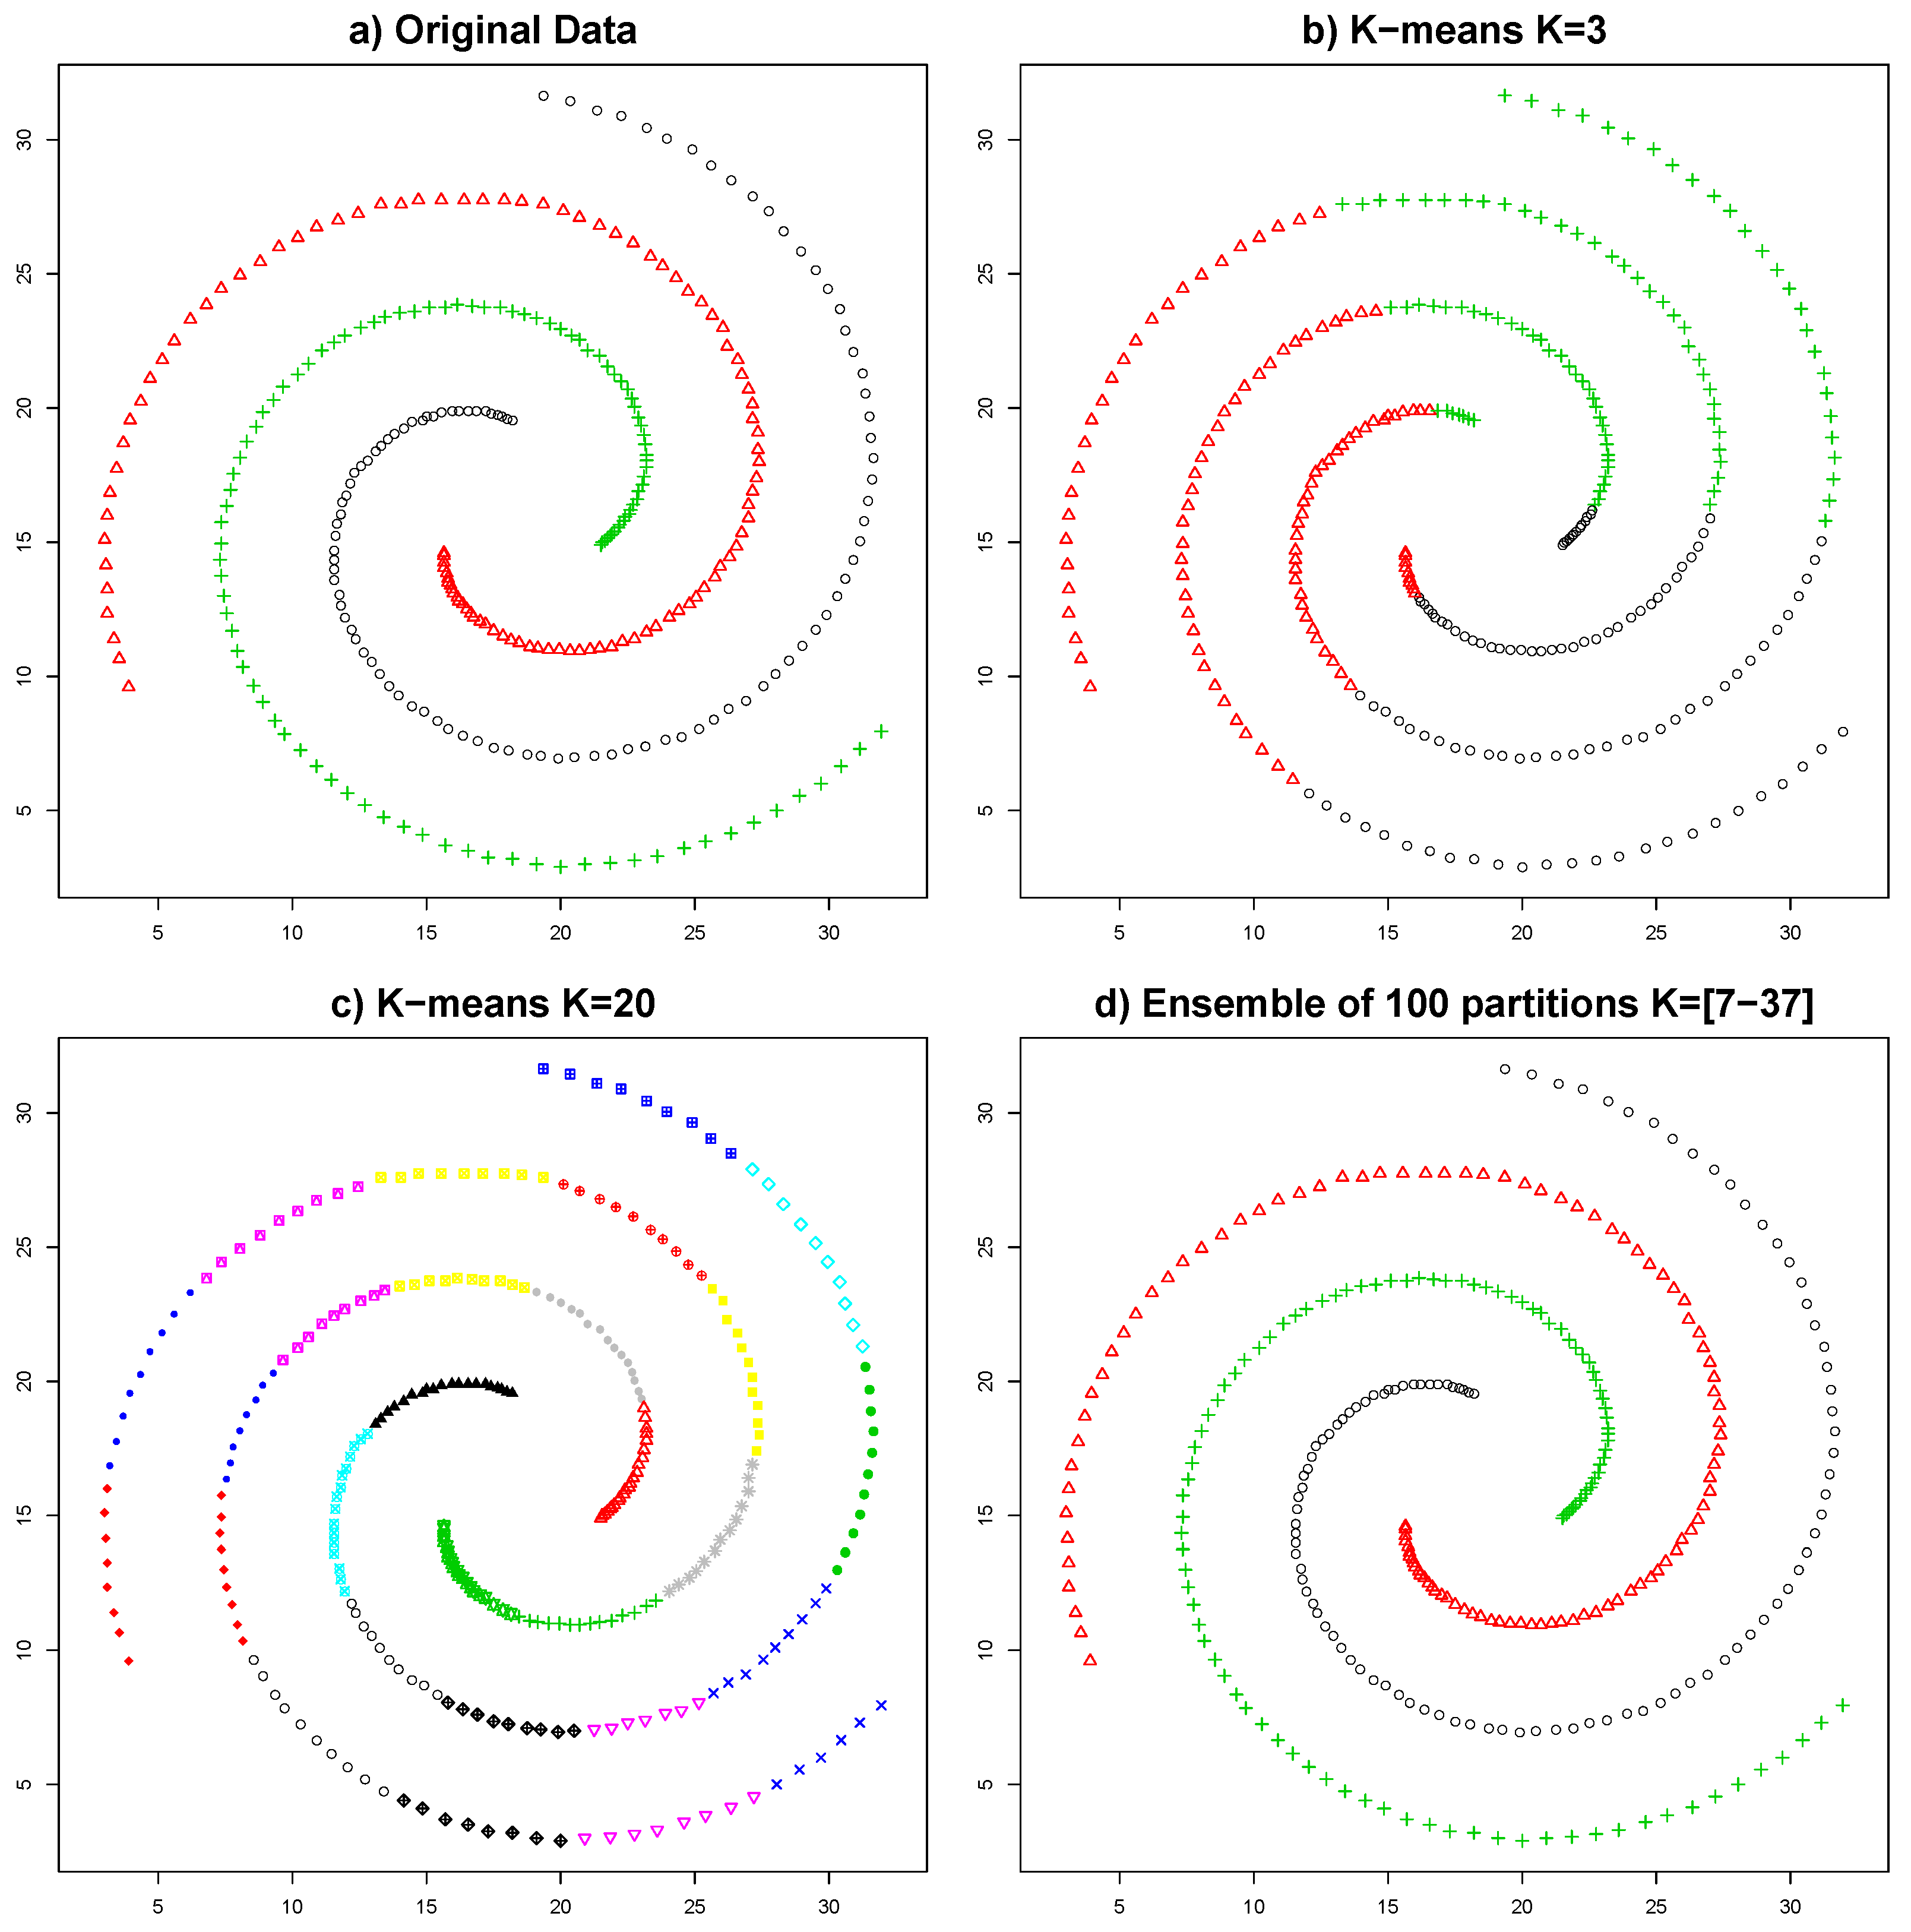
\includegraphics[width=7cm]{evidence accumulation clustering/figures/ensamble-example.png}
\end{center}

\note{
- Los métodos de clustering ensambles se basan en tomar \textbf{resultados} generados por \textbf{múltiples algoritmos} de clustering y llegar a un \textbf{consenso} que sea más correcto que los resultados individuales de los algoritmos utilizados. \\ %EAC es uno de ellos, y vamos a estar utilizandolo en esta ultima seccion. \\
- La idea detrás de \gls{EAC} es entonces \textbf{combinar los resultados de múltiples} clusterings en una \textbf{única partición de datos}, interpretando cada uno de estos resultados como una ``\textbf{evidencia independiente}'' de la organización de los datos, como puede apreciarse en la figura
}

\end{frame}

\begin{frame}
\frametitle{Evidence Accumulation Clustering}

\begin{itemize}
    \item<1-> Sea $X = {x_1, x_2,...,x_n}$ nuestro conjunto de datos donde $x_i \in R^d$ y $R^d$ es un espacio de $d$ features.
    \item<2-> Partición $P$ que encuentra $k$ clusters
    \item<3-> Dado $N$ algoritmos de clustering podemos entonces derivar $N$ particiones $P$
    \item<4-> Definimos al conjunto de estas particiones como:

    \begin{equation}
    \mathbb{P} = \{P^1, P^2,...,P^N\}
    \end{equation}
    
    \begin{multline}
    \hfill
        \begin{split}
        P^1 = \{C^1_1, C^1_2,...,C^1_{k_1}\}
        \end{split} \hfill \break
    \hdots \hfill \break
        \begin{split}
        P^N = \{C^N_1, C^N_2,...,C^N_{k_N}\}
        \end{split}
    \hfill
    \end{multline}

\note{
- \noindent donde $C^i_j$ es el cluster $j$th en la partición $P^i$, la cual tiene $k_i$ clusters. \\
- Además, dado $n^i_j$ como la cardinalidad de $C^i_j$, se cumple que $\sum_{j=1}^{k_i} n^i_j=n, \ \ i=1,...,N$. \\
- Cabe aclarar que los k pueden ser diferentes. \gls{EAC} no asume el número de clusters $k_i$ para cada partición obtenida $P^i$, por lo que cada $k_i$ pueden ser no sólo diferentes al número de clusters buscado por \gls{EAC}, sino que también entre sí.
}
\end{itemize}

\end{frame}

\iflong
\begin{frame}
\frametitle{Evidence Accumulation Clustering}

El objetivo es obtener una partición de datos ``óptima'' llamada $P^*$, que cumpla con las siguientes propiedades:
\begin{itemize}
    \item<1-> Consistencia con el ensamble de clusterings $\mathbb{P}$
    \item<2-> Robustez antes pequeñas variaciones en $\mathbb{P}$
    \item<3-> Ajuste con respecto al \gls{GT}
\end{itemize}

\note{
\begin{itemize}
    \item<1-> Significa que $\mathbb{P}$ sea el r\textbf{esultado de un acuerdo} entre las diferentes \textbf{partes encontradas} $P^i, i=1,...,N$.
    \item<2-> Los cantidad de clusters y los puntos pertenecientes a cada cluster en $P^*$ \textbf{deberían ser invariantes} ante \textbf{pequeñas perturbaciones} de $\mathbb{P}$.
    \item<3-> Los clusters encontrados deberán \textbf{coincidir} fuertemente con las \textbf{verdaderas etiquetas} de nuestros datos.
\end{itemize}
}

\end{frame}
\fi








\begin{frame}
\frametitle{Evidence Accumulation Clustering}

Tres problemas a resolver, que definen cada etapa del algoritmo de \gls{EAC}:

\begin{enumerate}
    \item  Cómo generamos el ensamble de particiones.
    \item  Cómo combinamos la evidencia.
    \item  Cómo extraemos una partición de datos (conjunto de clusters) consistente de la evidencia combinada.
\end{enumerate}

\note{
- Utilizaremos un algoritmo en particular, \textbf{k-means}, múltiples veces con \textbf{semillas diferentes} para generar el ensamble de clusters. \\
%- Para quienes no esten familiarizados con k-means es un algoritmo clásico del área de minería de datos. Dado un conjunto de k clusters buscados, asigna de forma aleatoria los centros de dichos clusters y los optimmiza iterativamente, asignando los puntos al centro del cluster más cercano en cada iteración. Similar Fuzzy clustering que explicamos antes. \\
%- Como el algoritmo es naturalmente inestable significa que podemos utilizar la variabilidad de múltiples corridas de k-means para llegar a un consenso, como se propone realizar con \gls{EAC}.
}

\end{frame}


\iflong
\begin{frame}
\frametitle{Evidence Accumulation Clustering}

El primer problema se puede abordar de las siguientes maneras:

\begin{enumerate}
\item<1-> Elección de representación de datos:
    \begin{enumerate}
     \item<2-> Empleando diferentes métodos de preprocesamiento y/o extracción de features.
     % , lo que resulta en diferentes representaciones de los datos o espacio de features.
     \item<3-> Explorando subespacios de la misma representación de datos.
     \item<4-> Perturbando los datos con métodos de bootstrapping o sampling.
     \end{enumerate}
\item<5-> Elección de algoritmos de clustering o parámetros de los algoritmos:
    \begin{enumerate}
     \item<6-> Aplicando diferentes algoritmos de clustering.
     \item<7-> Usando el mismo algoritmo pero con diferentes parámetros o inicializaciones.
     \item<8-> Explorando diferentes medidas de disimilitud para evaluar relaciones en nuestros datos.
     \end{enumerate}
\end{enumerate}

\note{
- Dos categorias sobre como resolver el problema. \\
- En este trabajo nos interesara aplicar lo mencionado en 2)b). Es decir, utilizaremos un algoritmo en particular, k-means, múltiples veces con semillas diferentes para generar el ensamble de clusters. \\
- Para quienes no esten familiarizados con k-means es un algoritmo clásico del área de minería de datos. Dado un conjunto de k clusters buscados, asigna de forma aleatoria los centros de dichos clusters y los optimmiza iterativamente, asignando los puntos al centro del cluster más cercano en cada iteración. Similar Fuzzy clustering que explicamos antes. \\
- Como el algoritmo es naturalmente inestable significa que podemos utilizar la variabilidad de múltiples corridas de k-means para llegar a un consenso, como se propone realizar con \gls{EAC}.
}

\end{frame}
\fi




\begin{frame}
\frametitle{Evidence Accumulation Clustering}

\begin{center}
    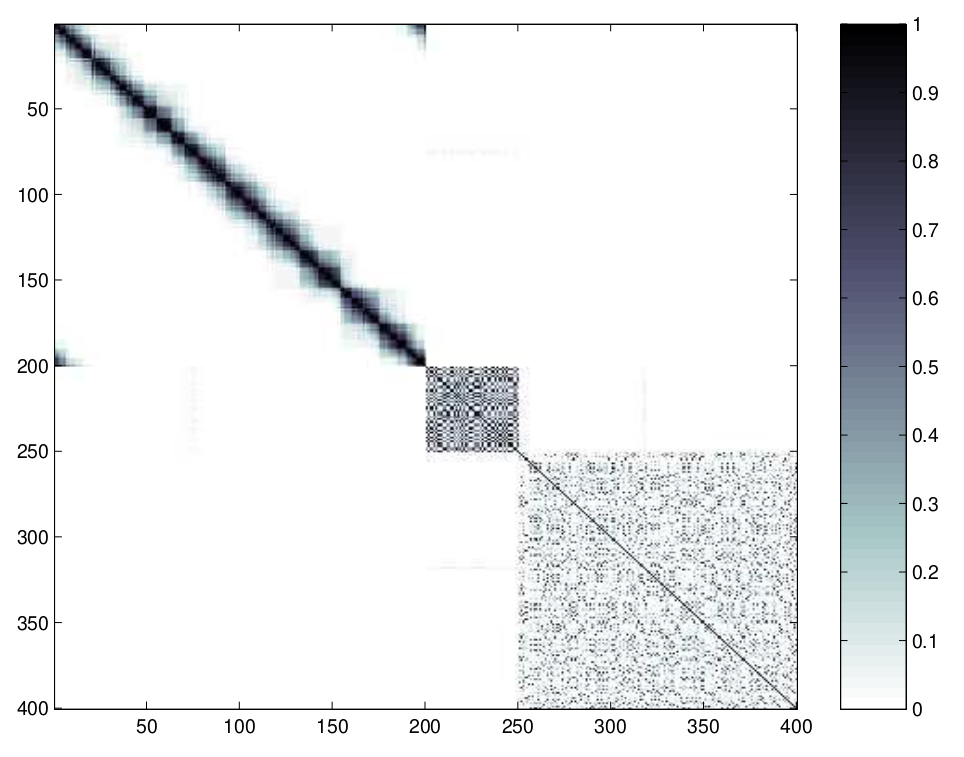
\includegraphics[width=6cm]{evidence accumulation clustering/figures/co-association matrix.png}
\end{center}

Mecanismo de votación y métrica de similitud

$$
C(i,j) = \frac{n_{ij}}{N}
$$

Donde $n_{ij}$ es el número de veces que el par de puntos $(i,j)$ son asignados al mismo cluster en $N$ particiones.

\note{
- Una vez obtenido el ensamble de particiones, pasaremos a combinar la información proveída de estos con una \textbf{matriz de co-asociación}. Esta nos permitirá \textbf{relacionar la información obtenida} con cada partición incluso si la cardinalidad varía entre ellas. \\
- Bajo la suposición de que dos puntos \textbf{pertenecen al mismo cluster} si se encontraron \textbf{en el mismo cluster repetidas veces} en el ensamble de particiones \\
- Una vez generada la \textbf{matriz de similitud} podemos aplicar \textbf{cualquier algoritmo de clustering sobre ésta}. El paper original opta por utilizar \textbf{clustering jerárquico aglomerativo} con \textbf{single o average} linkage, por lo que seguimos con eso.
}

\end{frame}


\begin{frame}
\frametitle{Librería utilizada}

\begin{center}

\href{https://pycombo.readthedocs.io/en/latest/}{https://pycombo.readthedocs.io/en/latest/}
\href{https://github.com/originalnicodr/combo}{https://github.com/originalnicodr/combo}

\end{center}

\note{
%- Aunque el paper original describe cómo la elección de donde cortar el dendrograma se realiza a partir de una medida de ``tiempo'' respecto a qué tanto se mantienen los clusters en el dendrograma antes de juntarse con otro, la librería mencionada nos da la opción de cortar el dendrograma en donde queramos para así obtener una partición de nuestros datos con la cantidad específica de clusters que buscamos. Esto nos es de especial utilidad para realizar los experimentos y comparaciones que venimos haciendo en los capítulos anteriores.\\
- Porque forkeamos la libreria 
}

\end{frame}


\begin{frame}
\frametitle{Abadi: Detección de 2 componentes}


\begin{columns}
\column{0.4\textwidth}
\begin{center}
\begin{itemize}
 \item $N = 500$
 \item k-means con $k_i = 100, i = 1, ..., N$.
\item Clustering Jerárquico aglomerativo con single linkage
\end{itemize}
\end{center}
\column{0.6\textwidth}
    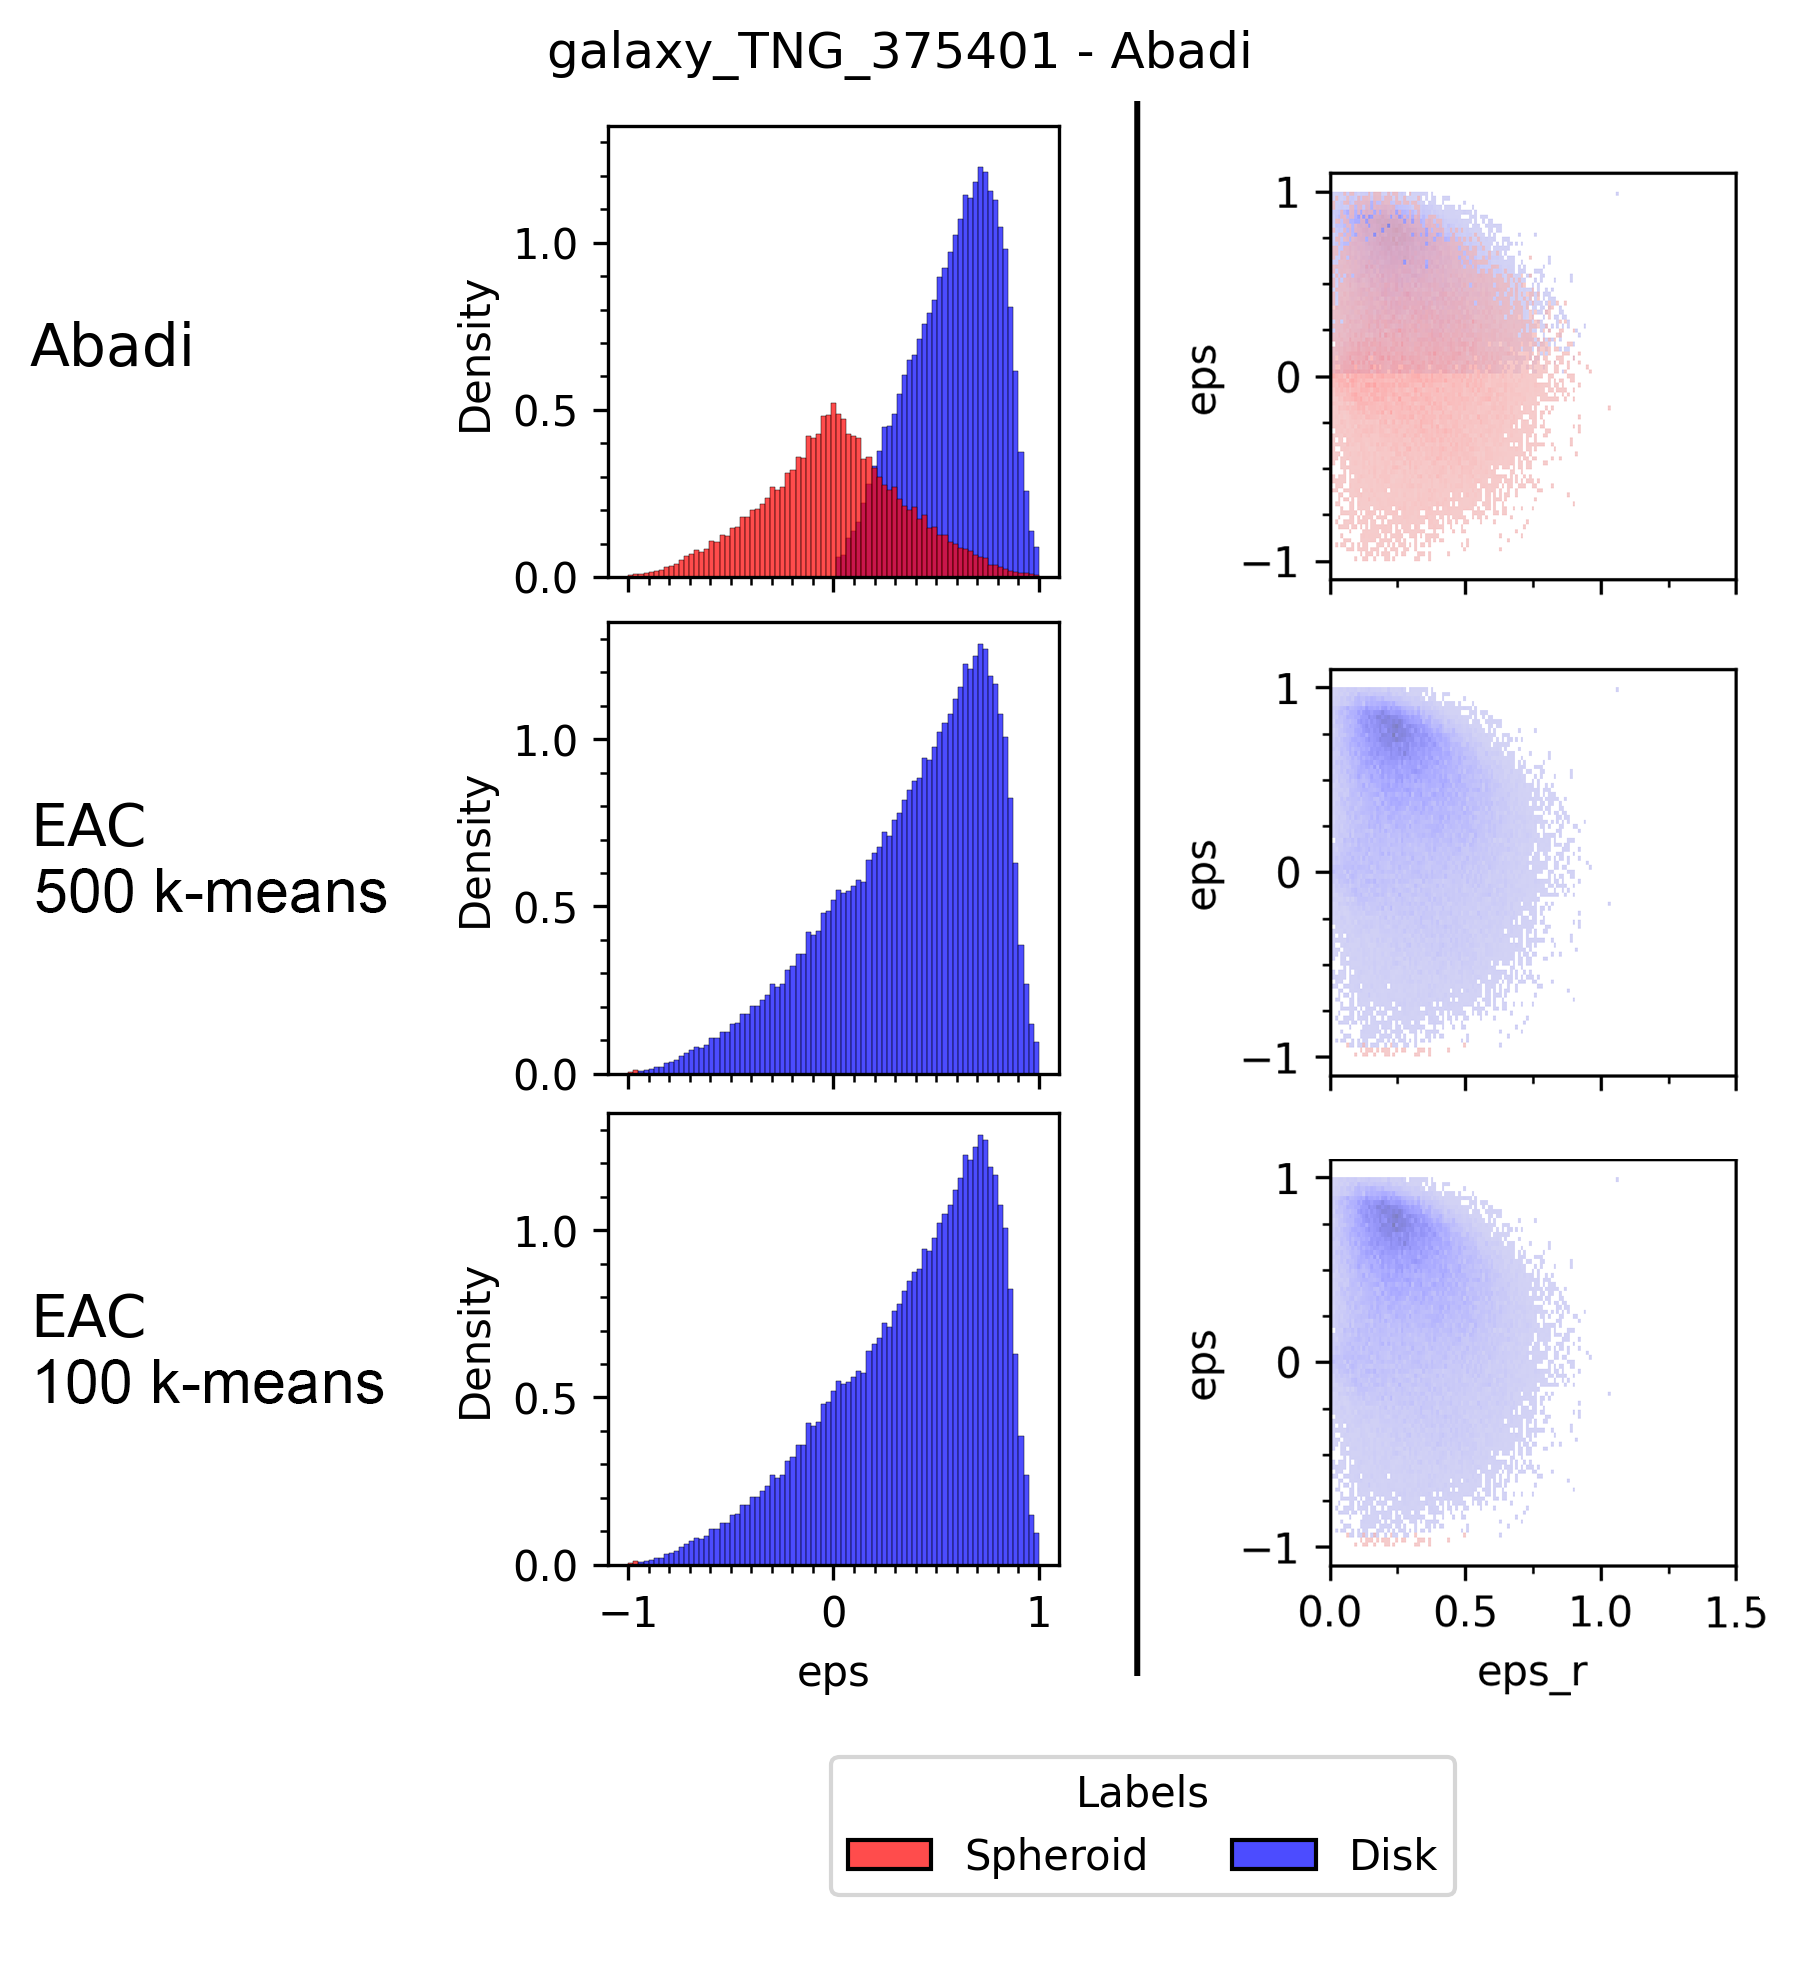
\includegraphics[width=6cm]{evidence accumulation clustering/figures/eac kmeans 500 vs 100.png}
\end{columns}

\note{
-  Habiamos probado con N = 500, pero \textbf{tardaba aun mas (cuatro dias)}, por lo cual optamos por reducir el numero de particiones a buscar a 100 \\
- La diferencia con N=500 era casi \textbf{imperciptible} \\
- Pero sigue siendo muy \textbf{caro computacionalmente}, por eso redujimos el analisis a tan solo \textbf{tres galaxias}, y dado los resultados feos que estamos viendo no valia la pena probarlos con todas (la falta de galaxias no es de gran impacto para nuestro analisis) \\
- \textbf{Por que da asi?} Antes de explicar: %Primero tenemos que ver la pinta que tienen los resultados de k-means (siguiente diapo)\\
}

\end{frame}


 \iflong
\begin{frame}
\frametitle{Abadi: Detección de 2 componentes}

\begin{center}
    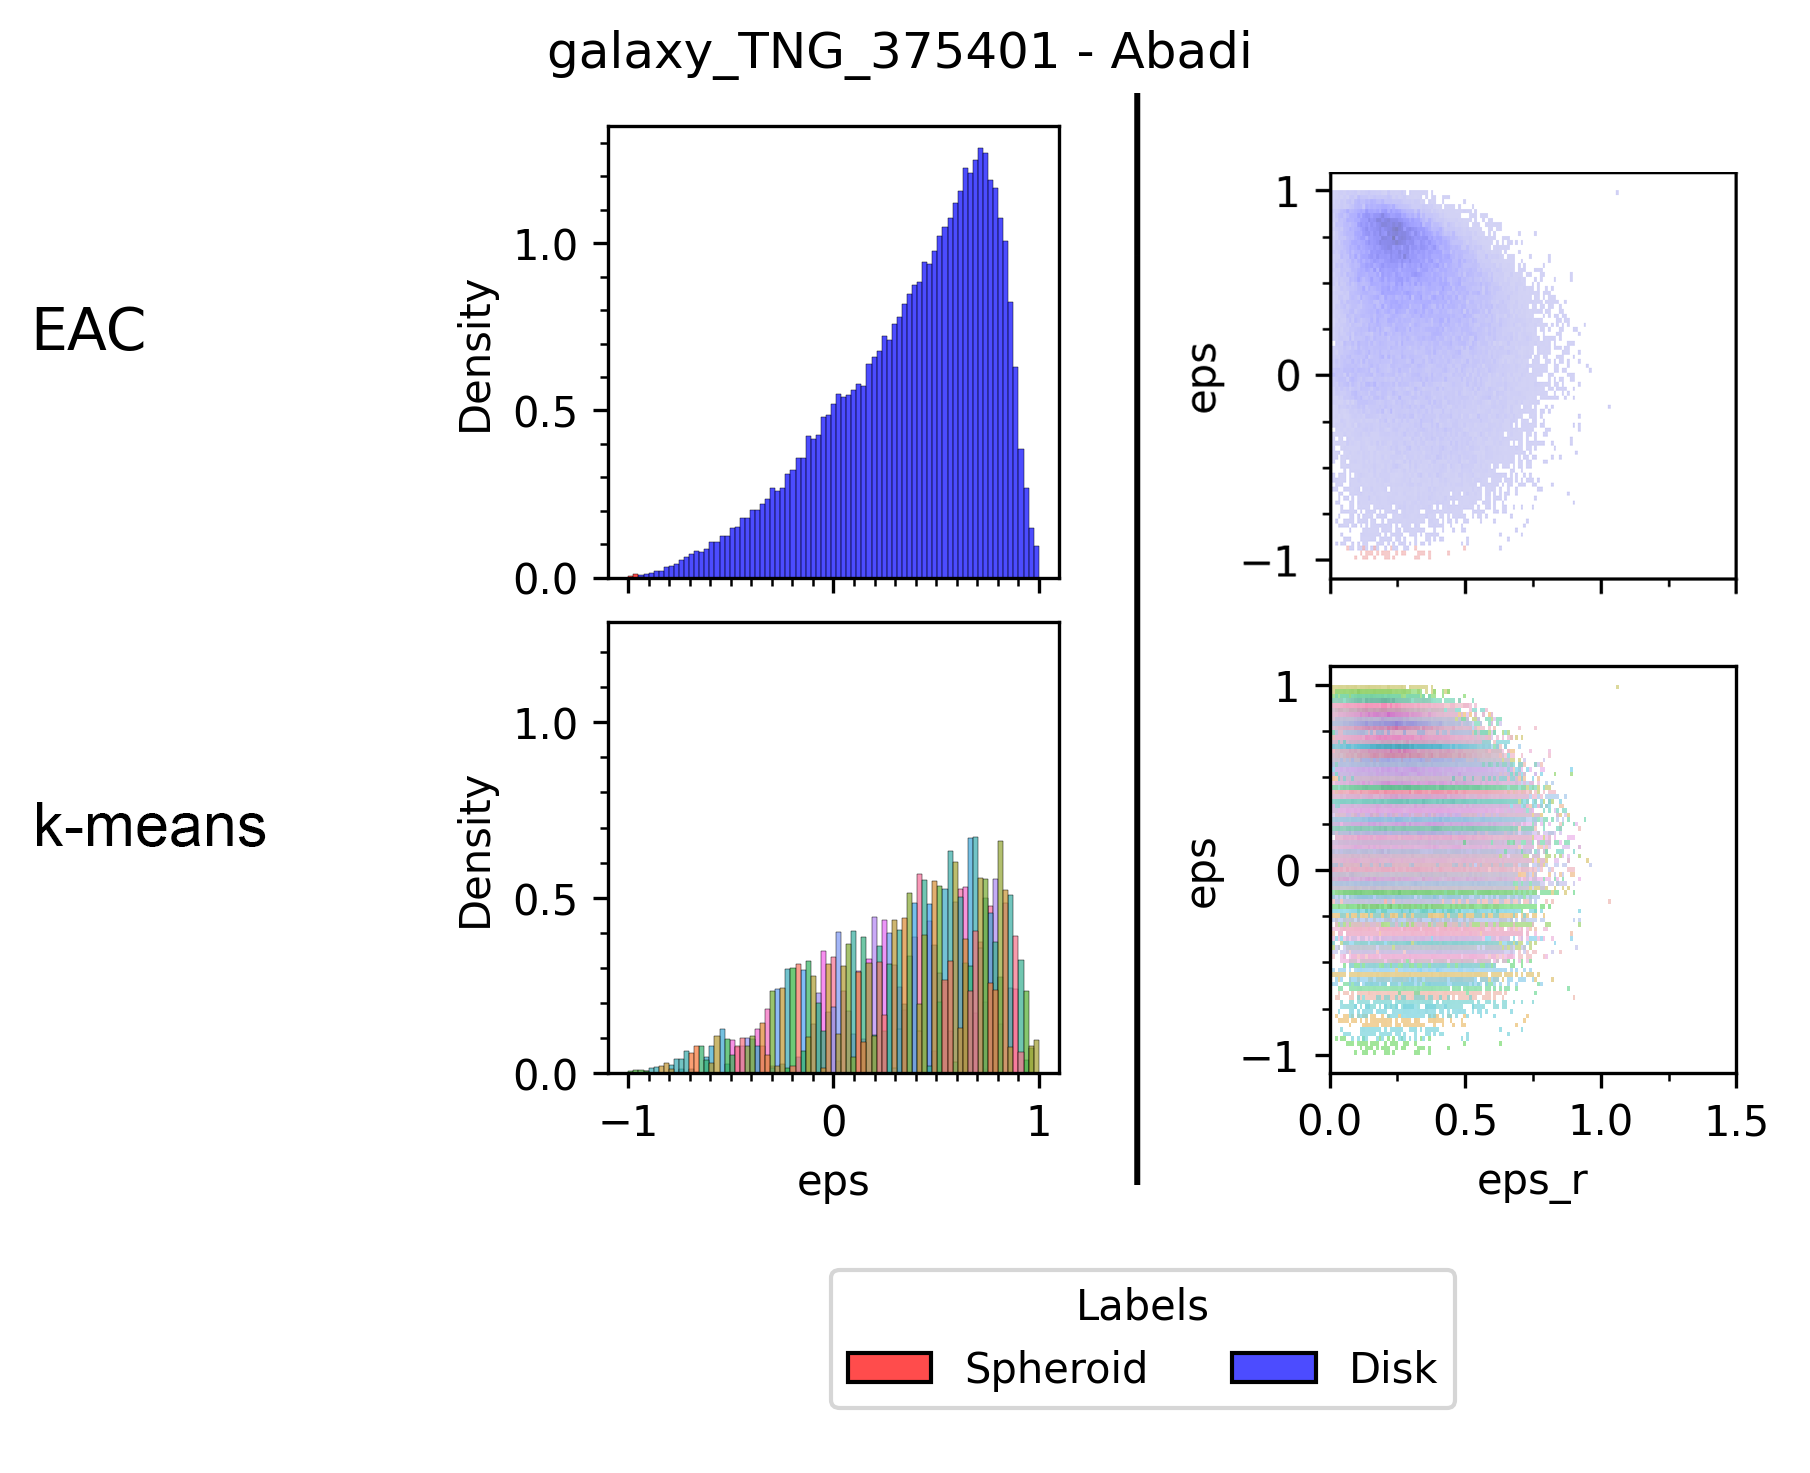
\includegraphics[width=8cm]{evidence accumulation clustering/figures/kmeans example.png}
\end{center}

\note{
- Pinta de estar separados en \textbf{lineas}, esto es porque solo usamos \textbf{eps} \\
- A medida que avanza HC en el ultimo paso del algoritmo de FCM, se van a ir \textbf{uniendo cada clusters adjacente} hasta llegar a los ultimos dos, separados por una linea \\
- Como funciona \textbf{single linkage}: \textbf{minimiza la menor distancia} posible entre dos clusters y los va uniendo \\
%- El mejor resultado hubiera requerido: las partículas alrededor del punto donde la densidad del Disco supera a la del Esferoide en Abadi no hayan compartido muchos clusters que ese punto haya particulas\\
- EAC prioriza en \textbf{fusionar lugares de mayor densidad}, ya que al aumentar la densidad de los puntos las probabilidades de encontrar clusters con metricas de disimilitud pequeñas se incrementa al utilizar single-linkage.  \\
- Por eso se va a un \textbf{extremo} la linea divisora \\
- Por lo feo que da, no vale la pena \textbf{remover outliers}, y ya de entrada no nos parece una buena alternativa \\
}

\end{frame}
\fi




\begin{frame}
\frametitle{AGMM: Detección de $=>$2 componentes}

\begin{center}
    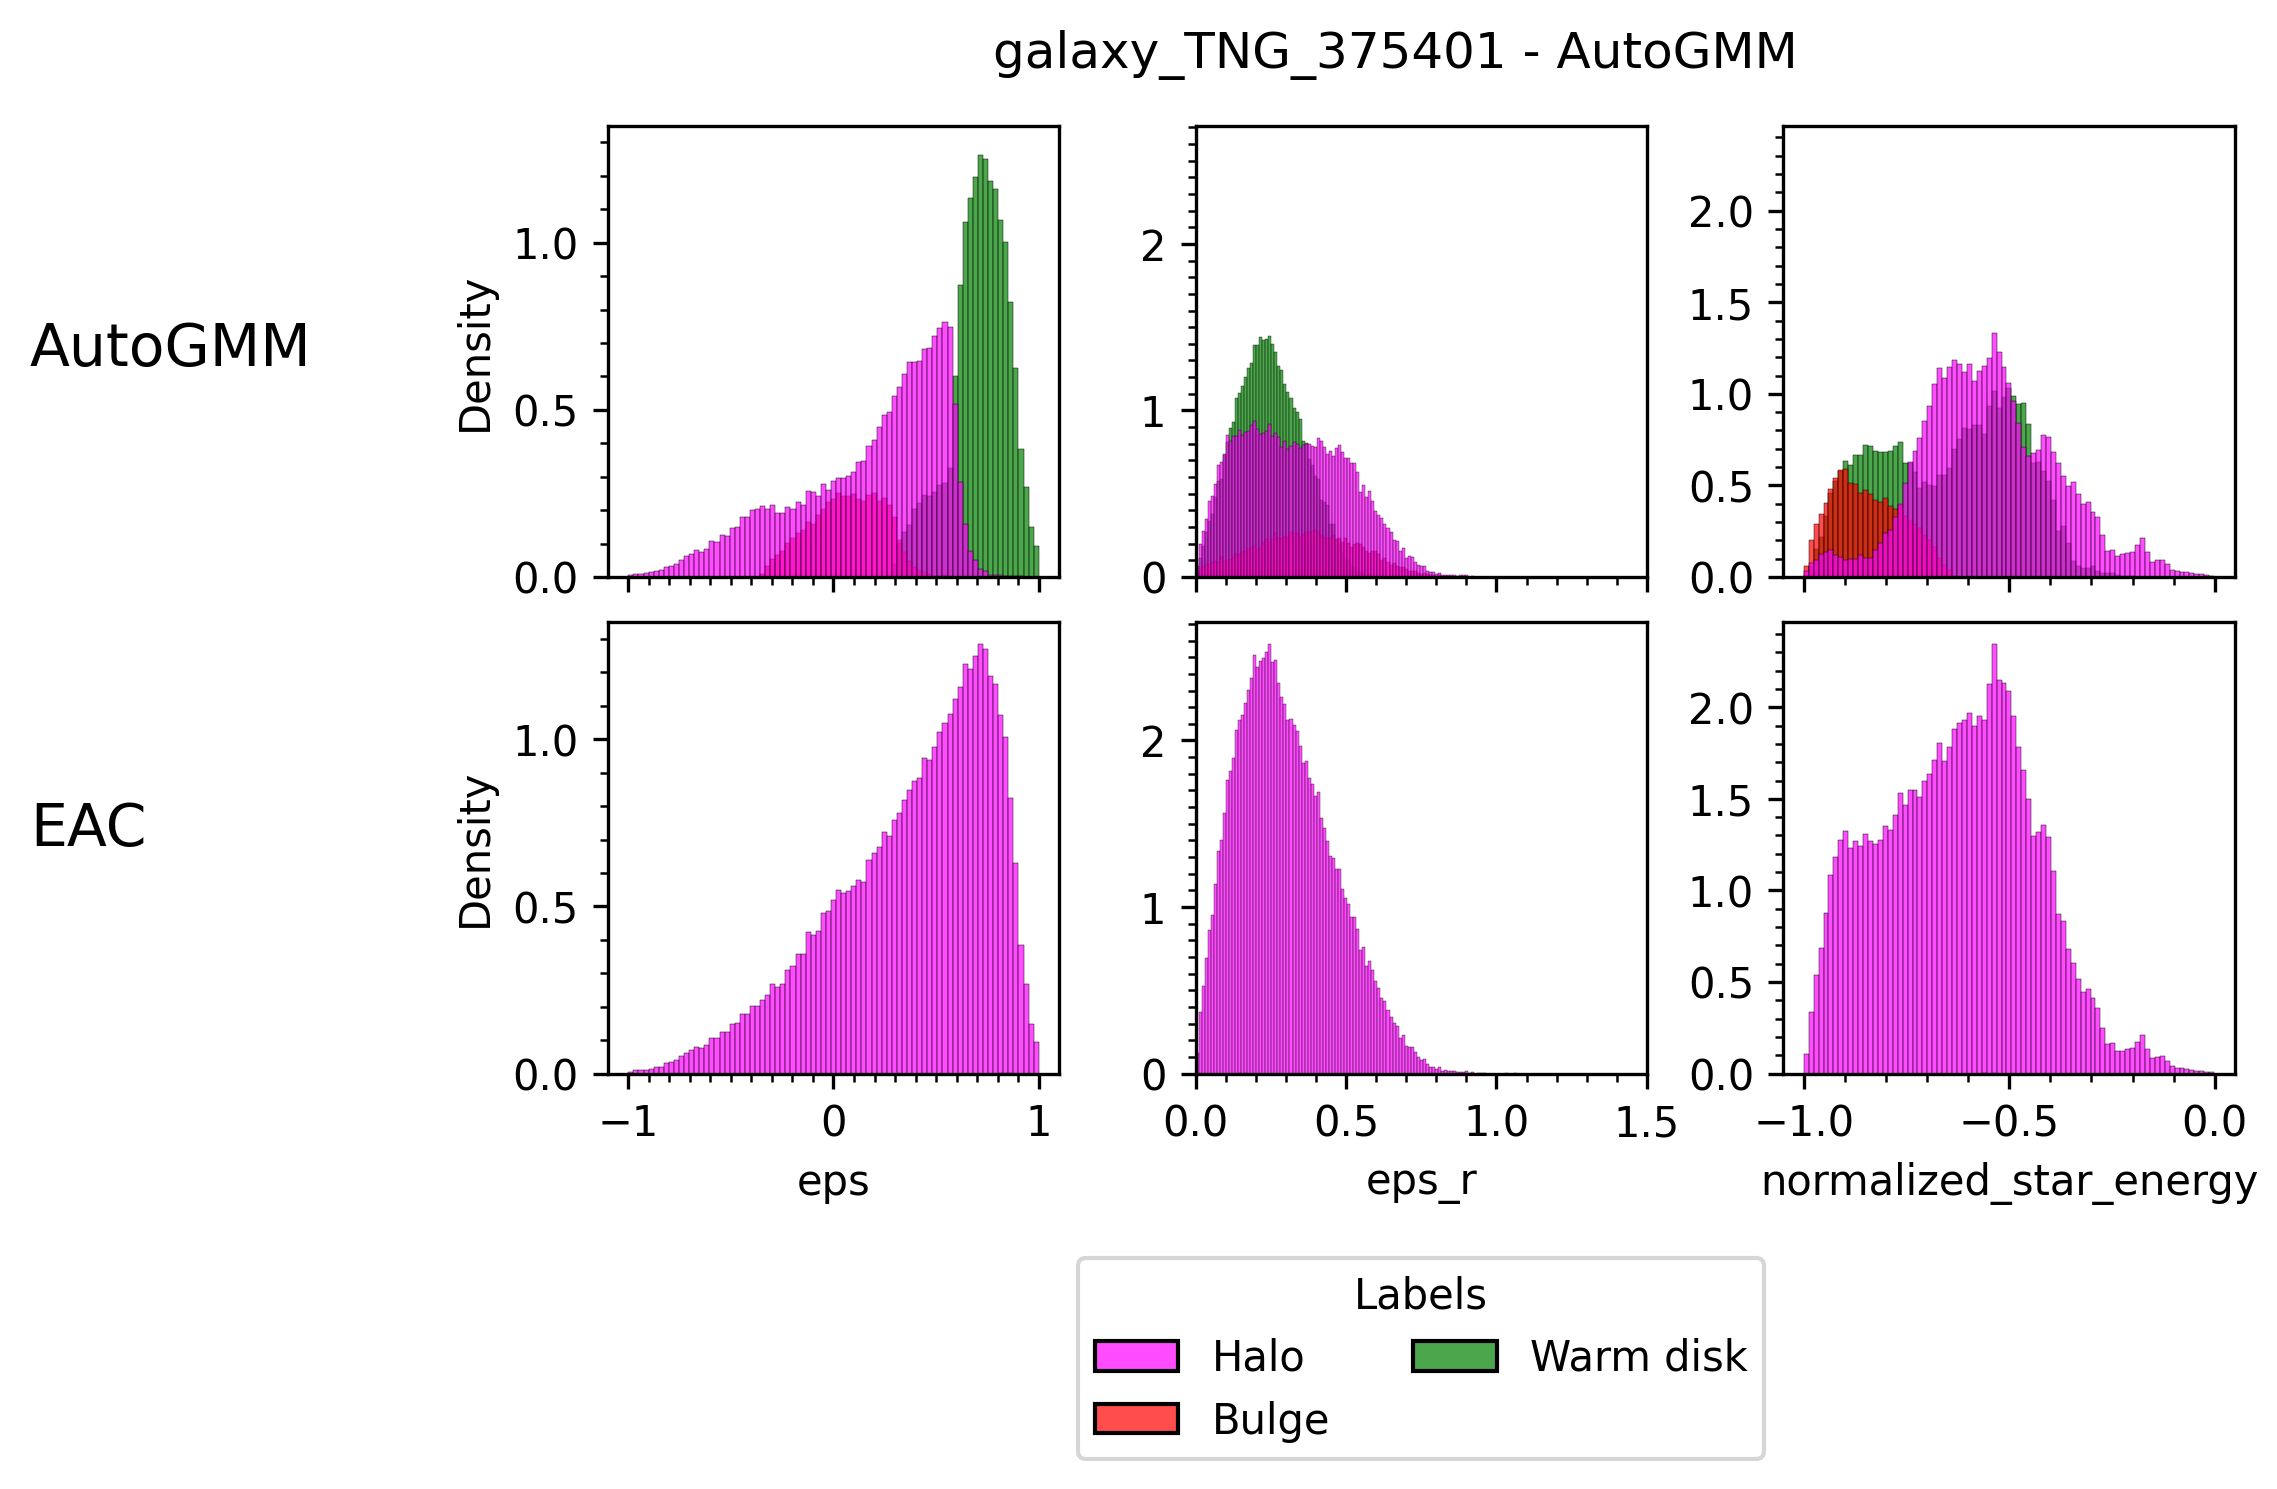
\includegraphics[width=10cm]{evidence accumulation clustering/figures/galaxy_TNG_375401 - eac - agmm - circ histogram.png}
\end{center}

\note{
- N = 100 denuevo \\
- seguimos con alto costo computacional \\
%- aca usamos todas las features, por lo que la razon explicada antes no debe estar aplicando aca \\
- Entendiendo eso, creemos que usar \textbf{valores MUY altos de k} puede entrometerse con encontrar los \textbf{patrones buscados en el dataset}. Resultando de esta manera en una matriz de consenso ruidosa y que \textbf{no captura las co-ocurrencias de los puntos}. \\
- Tambien descubrimos que uno de los experimentos que propone el paper original es \textbf{variar los valores de $k$} utilizados por cada k-means (dentro de las cotas adecuadas) en una misma corrida de \gls{EAC}, siendo esto al parecer \textbf{más robusto} que utilizar un $k$ fijo. \\%Se argumenta que usar un rango amplio de valores puede llegar a tener un efecto de promediado que nos lleve a la identificacion de la estructura verdadera de nuestros datos. \\
- \textbf{Ambas razones} pueden haber sido las causantes de la forma de los resultados obtenidos. Pero de igual manera con los tiempos de computos requeridos por el agoritmo, no habia tiempo para buscar estas cotas como hiperparametros. \\
- Con los experimentos realizados \textbf{no nos es posible recomendar eac} como alternativa para abadi ni para agmm.
}

\end{frame}
